%%%%%%%%%%%%%%%%%%%%%%%%%%%%%%%%%%%%%%%%%
% a0poster Landscape Poster
% LaTeX Template
% Version 1.0 (22/06/13)
%
% The a0poster class was created by:
% Gerlinde Kettl and Matthias Weiser (tex@kettl.de)
% 
% This template has been downloaded from:
% http://www.LaTeXTemplates.com
%
% License:
% CC BY-NC-SA 3.0 (http://creativecommons.org/licenses/by-nc-sa/3.0/)
%
%%%%%%%%%%%%%%%%%%%%%%%%%%%%%%%%%%%%%%%%%

%----------------------------------------------------------------------------------------
%	PACKAGES AND OTHER DOCUMENT CONFIGURATIONS
%----------------------------------------------------------------------------------------

\documentclass[a0,landscape]{a0poster}
\usepackage{multicol} % This is so we can have multiple columns of text side-by-side
\columnsep=100pt % This is the amount of white space between the columns in the poster
\renewcommand{\columnseprulecolor}{\color{LightBlue}}
\columnseprule=3pt % This is the thickness of the black line between the columns in the poster

\usepackage[svgnames]{xcolor} % Specify colors by their 'svgnames', for a full list of all colors available see here: http://www.latextemplates.com/svgnames-colors

\usepackage{times} % Use the times font
%\usepackage{palatino} % Uncomment to use the Palatino font

\usepackage{graphicx} % Required for including images
\graphicspath{{figures/}} % Location of the graphics files
\usepackage{booktabs} % Top and bottom rules for table
\usepackage[font=small,labelfont=bf]{caption} % Required for specifying captions to tables and figures
\usepackage{amsfonts, amsmath, amsthm, amssymb} % For math fonts, symbols and environments
\usepackage{wrapfig} % Allows wrapping text around tables and figures
\usepackage{comment} % Allows for commenting out large sections of text

\begin{document}


\begin{comment}
  ##### block 1: Abstract
(already figured out)
##### block 2: Introduction
- Cognitive distortions
- Cognitive-behavioral therapy (CBT)
- The original paper - https://aclanthology.org/2021.clpsych-1.17.pdf (Detecting Cognitive Distortions from Patient-Therapist Interactions)
- The problem of class imbalance in cognitive distortion predictive models
- The potential of generative AI models to address class imbalance
- The individual class classification vs binary classification
##### block 3: Initial Data Analysis
- The dataset used in this study
- Including the non-distorted class, running the data on tfidf and LinearSVC gives an F1-score of 0.32 as it only predicts the non-distorted and the 2nd highest distorted class
- Treating the problem as a binary classification problem and a multi-class classification problem for the 10 classes makes the models more useful
- The best F1-score for the multi-class classification problem is 0.21 using tfidf and LinearSVC
- The best F1-score for the binary classification problem is 0.73 using tfidf and SVC
- include graphs of the data, talk over with the professor which to include
	- show class imbalance
	- combine average scores for the no distortion and with no distortion data
	- heatmap of confusion matrix for best model
		- each of these available for binary and multi-class classification
	- show w/ no distortion heatmap
##### block 4: Sentence-BERT Embeddings
- Sentence-BERT (SBERT) embedding models
- Compare different models and their performance
- The best F1-score for the multi-class classification problem is 0.262 using the "intfloat/multilingual-e5-large-instruct" Sentence Transformer and LinearSVC
- The best F1-score for the binary classification problem is 0.756 using the "intfloat/multilingual-e5-large-instruct" Sentence Transformer with SVM
- ![[Pasted image 20240411161914.png]]
##### block 5: Generative AI Models
- Compare different generation techniques and their performance
- Compare different models and their performance
	- I have graphs for these:
	- average difference in F1 for each type of model and each type of generation technique and each type of classification (binary vs multiclass)
	- Probably same graphs as the initial graphs? Or could I roll all the graphs into 1? Or should I just focus on the change in score rather than the numbers themselves?
##### block 6: Results and Evaluation
- The best F1-score for the multi-class classification problem is 0.298 using the "intfloat/multilingual-e5-large-instruct" Sentence Transformer and MLPClassifier with hyperparameter tuning
- The best F1-score for the binary classification problem is 0.765 using the "intfloat/multilingual-e5-large-instruct" Sentence Transformer and SVM with hyperparameter tuning
- Include graphs of the data, talk over with the professor which to include
- have the classification report for each classification method (binary and multi-class)
	- support test count
##### Discussion
- Include the limitations of the study
- Inter-Annotator Agreement IAA score which posed a challenge
	- how it affects the generative AI - sampling data with generative AI might get it confused when it isn't clear which distortion is inside of the sample(s)
- If humans can't agree, it would pose a major challenge to classification AI
- Validating the original paper in separating the data
- ![[Pasted image 20240411163356.png]]
	- remove no distortion AI
	- table-ize this data
##### block 7: Conclusion
- The best model and the best F1-score
- Reiterate the problem and the goals
- Include the future work
  - different methods of text generation
	  - fine-tuning gpt2 like in [this paper](https://www.researchgate.net/publication/346813794_Exploring_the_Potential_of_GPT-2_for_Generating_Fake_Reviews_of_Research_Papers)
  	- playing around with many kinds of text generation inputs
  - different methods of categorization
  	- using gpt4 to categorize data instead of usual ML models
  	- manually implementing an F1 score for the multi class records
- Bring it all back to CBTherapy
	- How simply the binary classification is useful for a future system and would be a good first step for further analysis by a human
##### block 8: Acknowledgements
- include: QUEST Program, Dr. Lauren
##### block 9: References
- include: the main paper and the kaggle dataset, along with sklearn stuff like in the original paper, huggingface models
\end{comment}

\begin{minipage}[b]{0.55\linewidth}
\veryHuge \color{DarkOrange} \textbf{Exploring Generative A.I. for Addressing Class \\ Imbalance in Cognitive Distortion Predictive Models} 
\\
\color{Black}\\ % Title
%\Huge\textit{An Exploration of Complexity}\\[1cm] % Subtitle
\huge\\Connor Mulholland, BSCS Candidate; Paula Lauren, PhD, Professor, CoAS % Author(s)

 %Lawrence Technological University\\ % University/organization
\end{minipage}
%
\begin{minipage}[b]{0.25\linewidth}
\color{DarkSlateGray}\Large \textbf{Contact Information:}\\
Dept.\ of Mathematics and Computer Science\\ % Address
Science Building S121D\\
\\

\end{minipage}
%
\begin{minipage}[b]{0.18\linewidth}

\includegraphics[width=20cm]{LTU2.png} % Logo or a photo of you, adjust its dimensions here
\end{minipage}

\vspace{1cm} % A bit of extra whitespace between the header and poster content

%----------------------------------------------------------------------------------------

\begin{multicols}{4} % This is how many columns your poster will be broken into, a poster with many figures may benefit from less columns whereas a text-heavy poster benefits from more


%%%%%%%%%%%%%% ABSTRACT %%%%%%%%%%%%%%%%%%%%%%%%%%%%%
\color{Teal}
\section*{Abstract}
\color{black} 

Modern tools for natural language generation may enable Artificial Intelligence (AI) models to be better trained on imbalanced data by generating records for the 
minority classes. Specifically, the psychoanalytic cognitive distortion data is based on the irrational or biased ways of thinking which can contribute to negative 
emotions and behaviors, which are crucial in many types of therapy. We compare various types of Generative AI models for generating new records and the current 
limitations of these new models. We find that pretrained Sentence-Bidirectional Encoder Representations from Transformers (Sentence-BERT) embeddings 
(i.e., multilingual-e5-large-instruct) used to train a Support Vector Machine (SVM) classifier model yields the best binary results with an F1-score of 0.756. 
The addition of generated data using the Mistral-7B-Instruct-v0.2 model with recursive data generation on the binary classification task resulted in a marginal 
boost in performance with an F1-score of 0.765 using the same Sentence-BERT embeddings with SVM classification model.



%----------------------------------------------------------------------------------------
%	OBJECTIVES
%----------------------------------------------------------------------------------------

\color{Teal} % DarkSlateGray color for the rest of the content

%----------------------------------------------------------------------------------------
%	MATERIALS AND METHODS
%----------------------------------------------------------------------------------------



\color{Black}

\begin{comment}
\begin{center}\vspace{0.5cm}
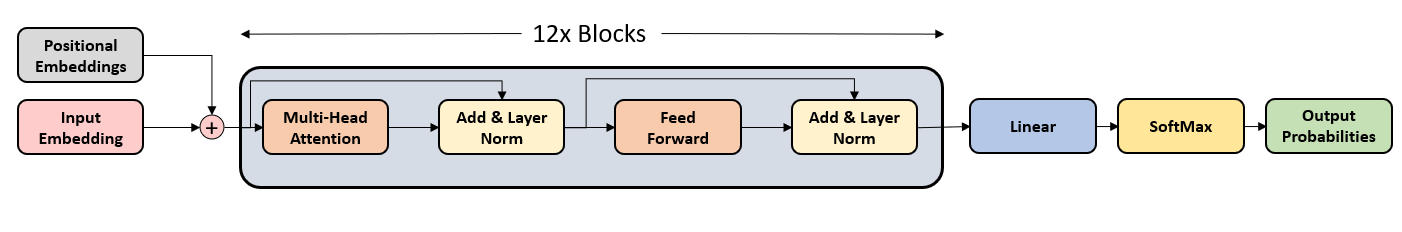
\includegraphics[width=0.99\linewidth]{GPT_1.png}
\captionof{figure}{\color{Teal} Generative Pre-trained Transformer Architecture.}
\end{center}\vspace{0.5cm}
\end{comment}

\color{Teal}

%%%%%%%%%%%%%% INTRODUCTION %%%%%%%%%%%%%%%%%%%%%%%%%%%%%
\section*{Introduction}
\color{Black}

Cognitive distortions are irrational or biased ways of thinking that can contribute to negative emotions and behaviors. Cognitive-behavioral therapy (CBT) is a common 
therapeutic approach that aims to help individuals identify and challenge these distortions. Detecting cognitive distortions from patient-therapist interactions is a 
challenging task that has been addressed in recent research. The paper who first utilized this data\cite{original_paper} uses a dataset of patient-therapist interactions to train a 
model to detect cognitive distortions. However, the dataset is highly imbalanced, with the majority of the data belonging to the non-distorted class. This class 
imbalance poses a challenge for training accurate predictive models. Generative AI models have the potential to address class imbalance by generating synthetic data 
for the minority classes. In this study, we explore the use of generative AI models to address class imbalance in cognitive distortion predictive models. We compare 
the performance of different generative AI models and classification algorithms on the task of detecting cognitive distortions from patient-therapist interactions. 
We consider both binary and multi-class classification tasks and evaluate the models using F1-score as the performance metric.

%%%%%%%%%%%%%% INITIAL DATA ANALYSIS %%%%%%%%%%%%%%%%%%%%%%%%%%%%%
\color{Teal}
\section*{Initial Data Analysis}
\color{Black}

We use a dataset of patient-therapist interactions to train our models. The dataset contains 10 classes of cognitive distortions, with the majority of the data belonging 
to the non-distorted class. We first treat the problem as a binary classification task, where we combine all the distorted classes into a single class and compare the 
performance of different classification algorithms. We use the Term Frequency-Inverse Document Frequency (tf-idf) vectorizer to convert the text data into numerical 
features and train a Linear Support Vector Classifier (LinearSVC) on the data. The best F1-score for the binary classification task is 0.73 using tf-idf and LinearSVC. 
We then treat the problem as a multi-class classification task and compare the performance of different classification algorithms. The best F1-score for the multi-class 
classification task is 0.21 using tf-idf and LinearSVC. The addition of the non-distorted class to the multi-class classification task resulted in a marginal improvement 
in performance, with an F1-score of 0.32 using tf-idf and LinearSVC.

\begin{center}\vspace{0.5cm}
	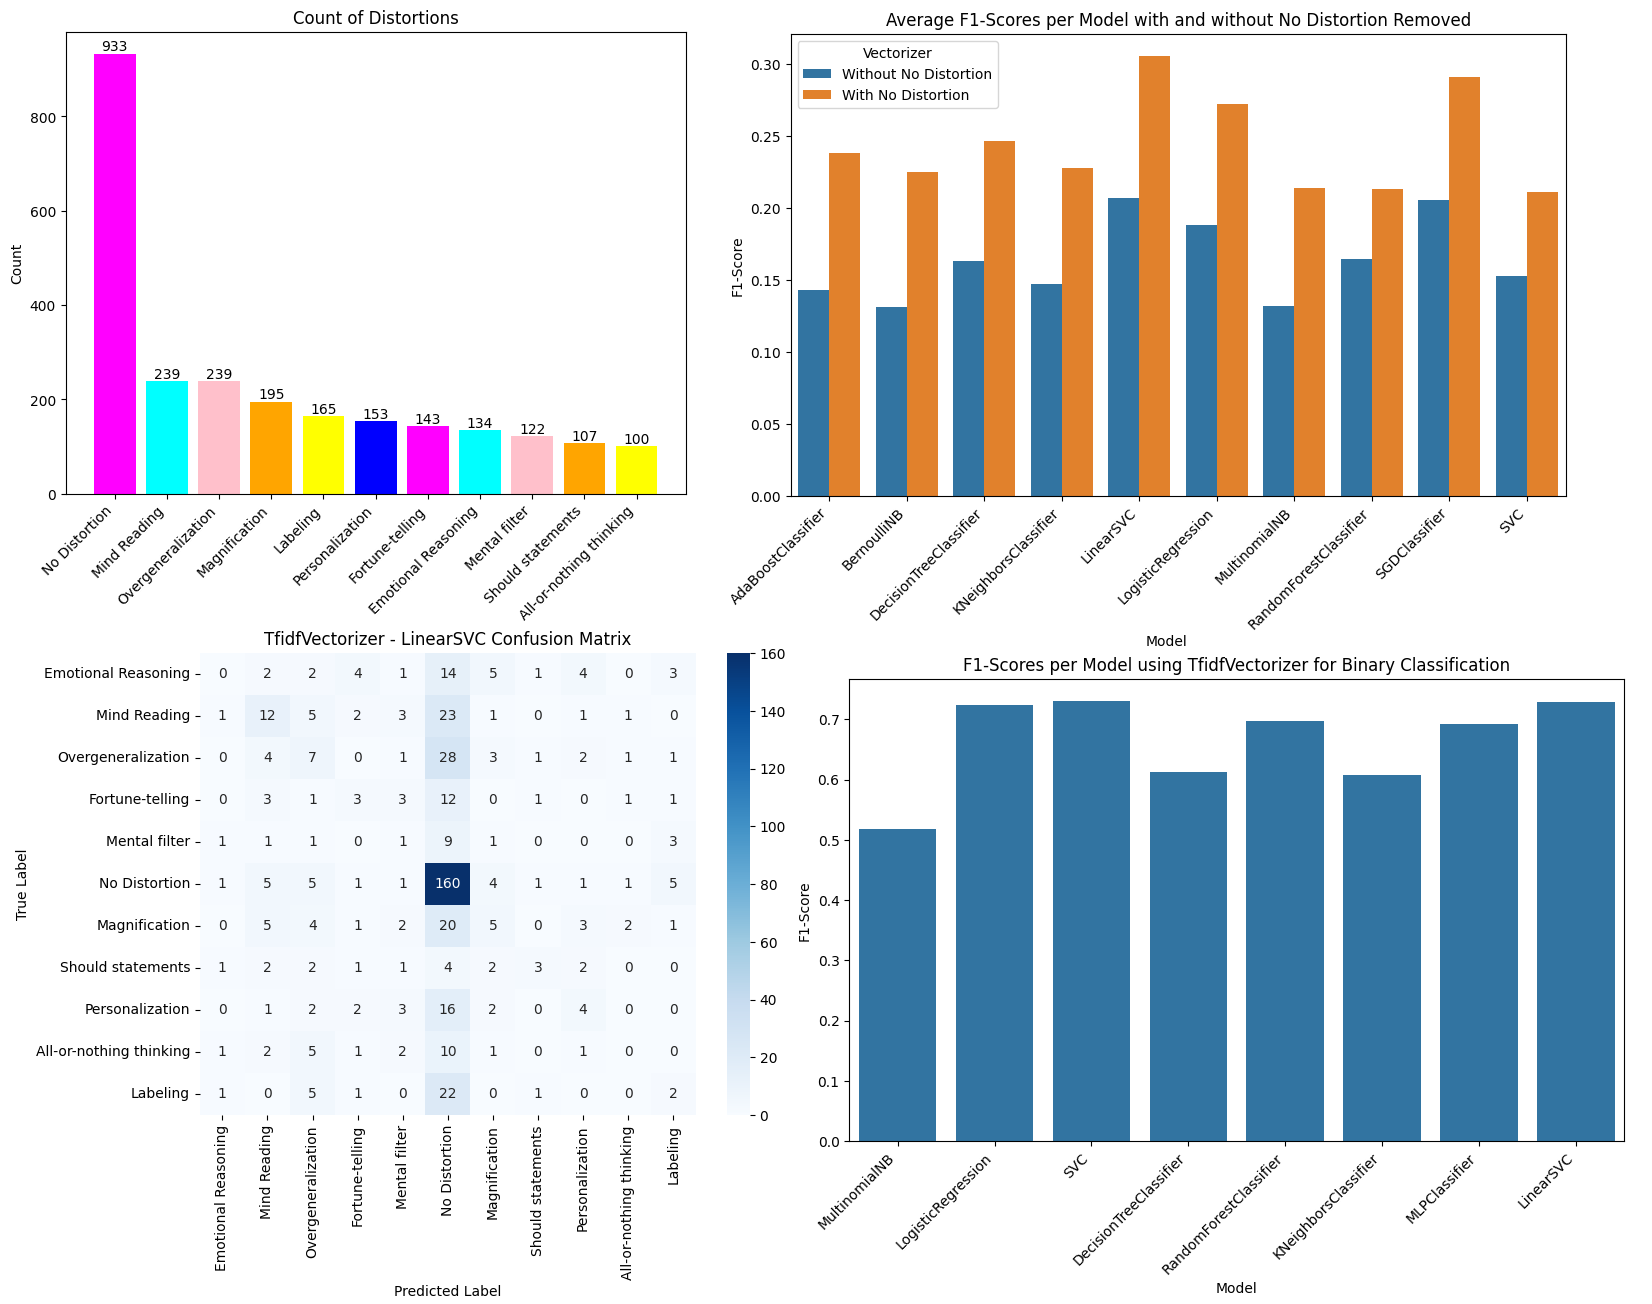
\includegraphics[width=0.99\linewidth]{figures/1stFour.png}
	\captionof{figure}{\color{Teal} (Top-Left) Class Imbalance, (Top-Right) Average F1-Scores with and without No Distortion data, (Bottom-Left) Confusion Matrix of best model with No Distortion data, (Bottom-Right) F1 Scores for Binary Classification}
\end{center}\vspace{0.5cm}

%%%%%%%%%%%%%% SBERT EMBEDDINGS %%%%%%%%%%%%%%%%%%%%%%%%%%%%%
\color{Teal}
\section*{Sentence-BERT Embeddings}
\color{Black}

Sentence-BERT (SBERT) is a variant of the BERT model that is specifically trained to generate sentence embeddings. We compare the performance of different SBERT models 
on the task of detecting cognitive distortions from patient-therapist interactions. We use the Sentence Transformer library to generate SBERT embeddings for the text 
data and train different classification algorithms on the embeddings. The best F1-score for the multi-class classification task is 0.262 using the 
"intfloat/multilingual-e5-large-instruct" SBERT model and LinearSVC. The best F1-score for the binary classification task is 0.756 using the 
"intfloat/multilingual-e5-large-instruct" SBERT model with SVM.

\begin{center}\vspace{1cm}
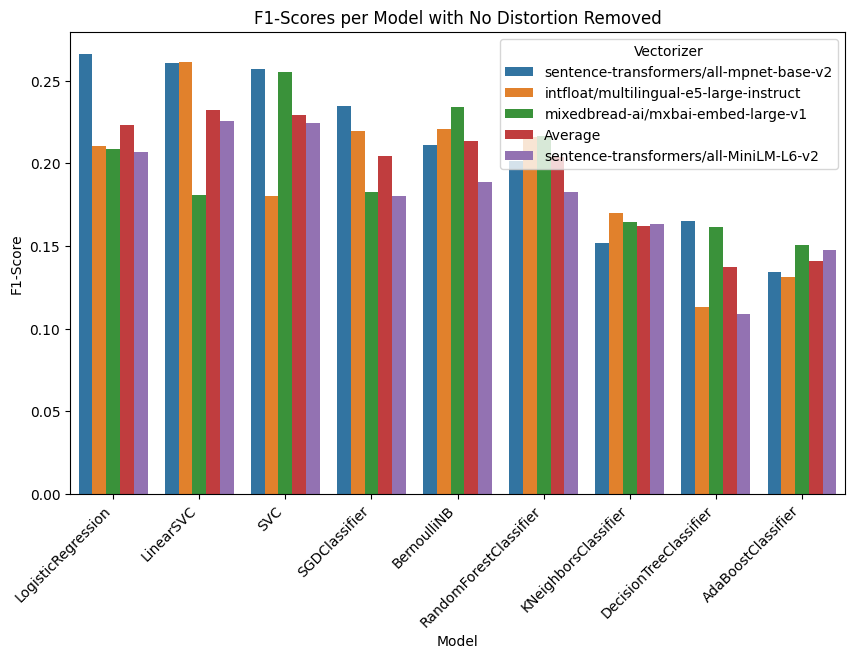
\includegraphics[width=0.99\linewidth]{figures/F1ScoresInitSBERT.png}
\captionof{figure}{\color{Teal} F1-Scores for SBERT Models}
\end{center}\vspace{1cm}

\color{Black}

%%%%%%%%%%%%%% GENERATIVE AI MODELS %%%%%%%%%%%%%%%%%%%%%%%%%%%%%
\color{Teal}
\section*{Generative AI Models}
\color{Black}

We explore the use of generative AI models to address class imbalance in cognitive distortion predictive models. We compare the performance of different generation 
techniques, including fine-tuning GPT-2 models and recursive data generation. We also compare the performance of different classification algorithms on the generated data. 
The best F1-score for the multi-class classification task is 0.285 using the "intfloat/multilingual-e5-large-instruct" SBERT model and MLPClassifier with hyperparameter 
tuning. The best F1-score for the binary classification task is 0.765 using the "intfloat/multilingual-e5-large-instruct" SBERT model and SVM with hyperparameter tuning. 
The addition of generated data using the Mistral-7B-Instruct-v0.2 model with recursive data generation on the binary classification task resulted in a marginal boost 
in performance with an F1-score of 0.765 using the same SBERT embeddings with SVM classification model.

\begin{center}
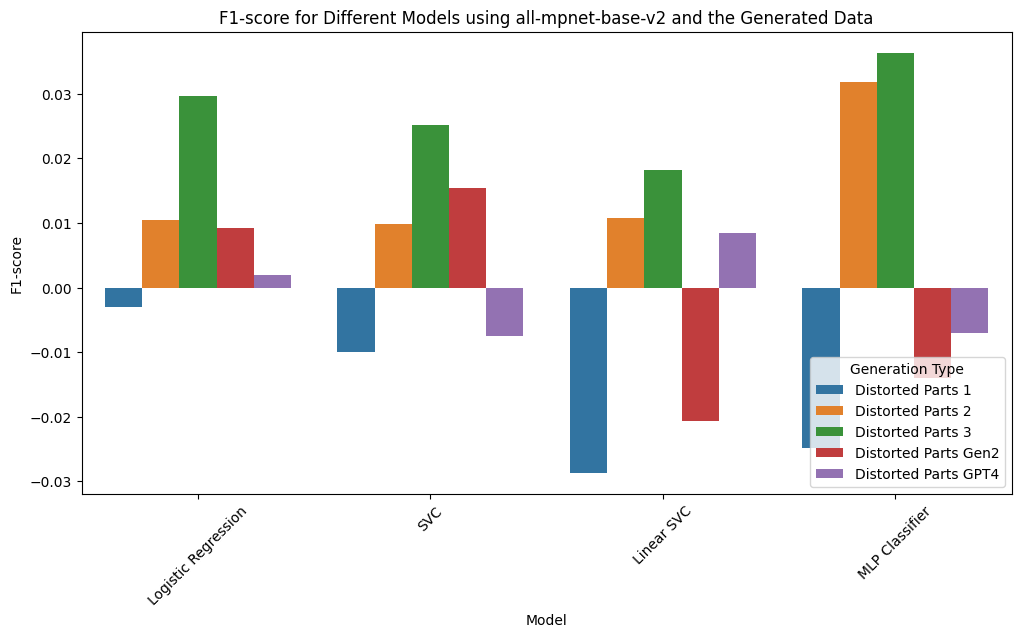
\includegraphics[width=0.60\linewidth]{figures/generatedDataDiffDiff.png}
\captionof{figure}{\color{Teal} Fine Tuning Architecture}
\end{center}\vspace{1cm}

%%%% Subsection
\color{Teal}
\subsection*{The Fine-Tuning Process}
\begin{center}
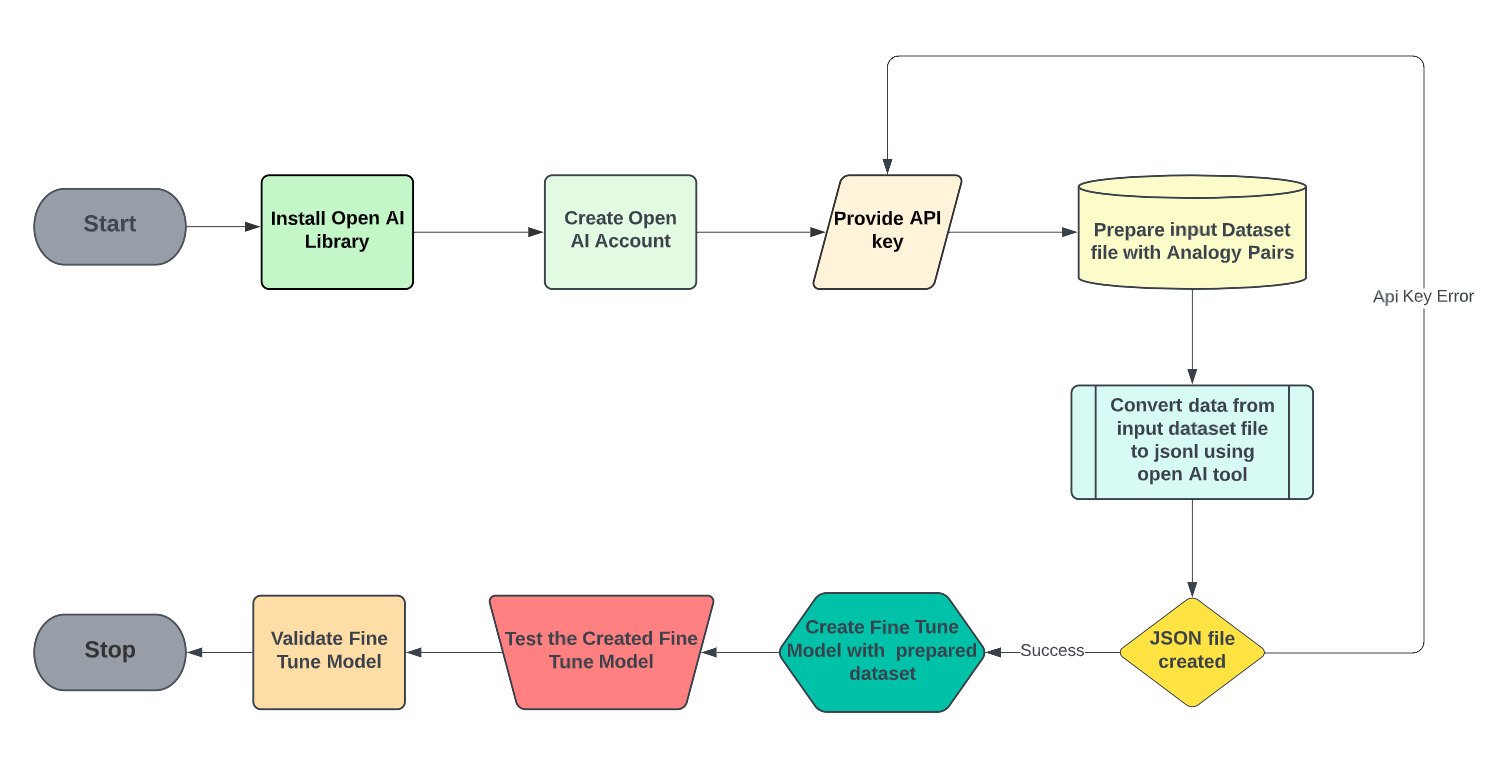
\includegraphics[width=0.99\linewidth]{FlowChart.png}
\captionof{figure}{\color{Teal} Fine-Tuning Process Step-by-Step}
\end{center}\vspace{1cm}

\color{black}
The below illustration depicts the outcome of the fine-tuned model for the example elaborated in Figure 3.

Bananas are more closely related to avocados than to limes because both belong to the same plant family, called the Musaceae family.
\vspace{0.5cm}

As illustrated in Figure 6, fine-tuning a pre-trained language model can enhance its performance on a given task or dataset. By adjusting the pre-trained model on a specific dataset, the model can learn the nuances and subtleties of the data and perform more accurately and meaningfully.
\vspace{0.5cm}

In addition to the example shown in Figure 6, there are several other examples where fine-tuning has demonstrated impressive results. These instances are shown in the table below.

%%%% Table example
 \begin{center}\vspace{1cm}
\centering
\begin{tabular}{c|c|r}
\toprule
\textbf{Prompt}  &  \textbf{GPT}  & \textbf{Fine-Tuned} \\
\midrule
Yellow is to banana and green is to  &    Lime  & Avocado\\ \hline
Computer is to software and brain is to   &   Hardware   & Cognition\\ \hline
Knife is to cooking as screwdriver is to  &   DIY projects  & Repair \\ \hline
Shovel is to gardening as keyboard is to &   Computing   & Typing\\ \hline
Microphone is to sound as camera is to &    Light  & Images\\ \hline
Car is to engine as computer is to &   Keyboard   & Processor\\ \hline
Glacier is to iceberg as stream is to &   Rock   & River \\ \hline
Rust is to decay as charcoal is to &   Burning   & Ash\\ \hline
Forgiveness is to healing as medicine is to &   Health    & Recovery \\ \hline
\bottomrule
\end{tabular}
\captionof{table}{\color{Teal} {  Analysis of Fine-Tuned Model }
\label{origCounts}}
\end{center}\vspace{1cm}

%%%%%%%%%%%%%% RESULTS AND EVALUATION %%%%%%%%%%%%%%%%%%%%%%%%%%%%%
\color{Teal}
\section*{F1-Score Results Analysis}
\color{Black}


\begin{itemize}
  \item The challenge at hand is that OpenAI, a leading AI research organization, will be offering a limited-time free subscription to their API service. This subscription will only be available for a duration of three months and will come with a limited amount of credits for using the API and fine-tuning it. Users may need to carefully plan and prioritize their use of the API within the allotted time and credit. 
  \item During the process of fine-tuning a learning model, users may have to wait for an unpredictable amount of time for the model to be fully trained. This wait time can vary depending on several unknown factors, and can range from minutes to hours or even days. This unpredictability can be a frustrating and time-consuming challenge for users who need to balance their fine-tuning activities with other tasks and responsibilities.
\end{itemize}



\color{Teal}
\section*{Conclusion}
\color{Black}



In conclusion to our research, fine-tuning is a crucial process that can significantly improve the performance of pre-trained NLP models on specific tasks or domains. Our findings show that the pre-trained GPT models can benefit from fine-tuning, as they are trained on massive datasets with broad contexts and may not generalize well on specific tasks or domains. Fine-tuning allows the models to adapt to the target task or domain by learning the relevant patterns and relationships from a smaller dataset, leading to higher accuracy and efficiency.

\vspace{1cm}
Our analysis of the fine-tuning results shows that the fine-tuned GPT models outperformed their pre-trained large language model and achieved better results in the analogy task. This indicates the effectiveness of the fine-tuning process in improving the models' performance on specific tasks or domains.

%----------------------------------------------------------------------------------------
%	FORTHCOMING RESEARCH
%----------------------------------------------------------------------------------------

%\section*{Forthcoming Research}

%Vivamus molestie, risus tempor vehicula mattis, libero arcu volutpat purus, sed blandit sem nibh eget turpis. Maecenas rutrum dui blandit lorem vulputate gravida. Praesent venenatis mi vel lorem tempor at varius diam sagittis. Nam eu leo id turpis interdum luctus a sed augue. Nam tellus.

 %----------------------------------------------------------------------------------------
%	REFERENCES
%----------------------------------------------------------------------------------------

%\nocite{*} % Print all references regardless of whether they were cited in the poster or not
%\bibliographystyle{plain} % Plain referencing style
%\bibliography{sample} % Use the example bibliography file sample.bib

%----------------------------------------------------------------------------------------

\color{Teal}
\section*{Acknowledgements}
\color{Black}

We would like to acknowledge the support of the QUEST Program and Dr. Lauren for their guidance and assistance throughout this research project.

\color{Teal}
\begin{thebibliography}{9}
\color{Black}

\bibitem{original_paper}
Detecting Cognitive Distortions from Patient-Therapist Interactions. (2021). \textit{ACL Anthology}. Retrieved from https://aclanthology.org/2021.clpsych-1.17.pdf
\end{thebibliography}

\end{multicols}
\end{document}